\chapter{Adding Reserve Items}
\label{ch:add}
\ares allows for items of different types. This chapter will cover all these types in the order of Book~(\autoref{sec:book}), Book Chapter or Article~(\autoref{sec:bchapterandart}) and Video~(\autoref{sec:video}). 

At the moment, we suppose you are already on the ``Course Home'' page~(\autoref{sec: course page}). 

If you just rushed to this chapter after logging in, you can select {\imp Current and Upcoming Courses} under \textbf{Instructor Tools}. Find the desired course and click \uline{View Course}. Then you are there!

\vspace*{4ex}
\begin{figure}[h]
    \centering
    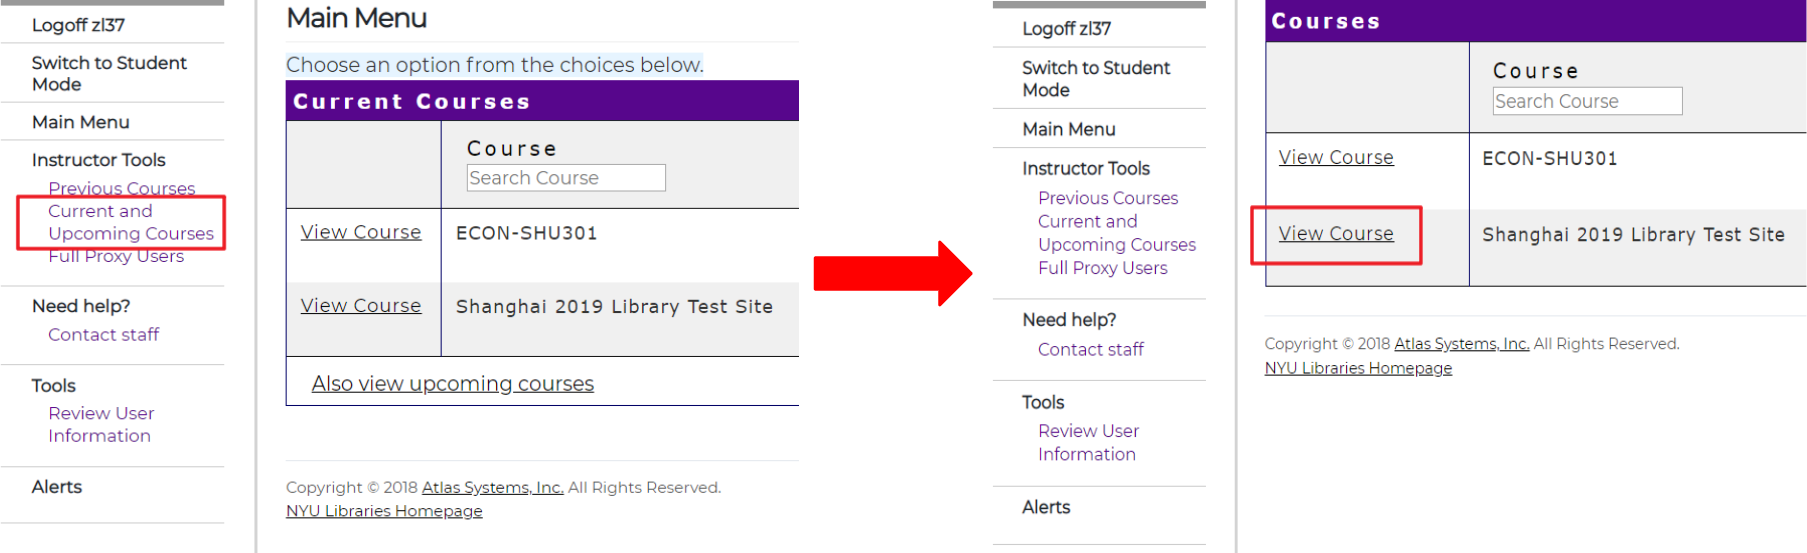
\includegraphics[width=\textwidth]{step}
    \caption{Get to the course page}
    \label{fig:go to course}
\end{figure}
\vspace*{2ex}

Once in the desired course, click on {\imp Add Reserve Items} under the \textbf{Instructor Course Tools} on the right side bar, and now you are able to select the appropriate course form: Article, Chapter, Book and Video. 

\vspace*{4ex}
\begin{figure}[h]
    \centering
    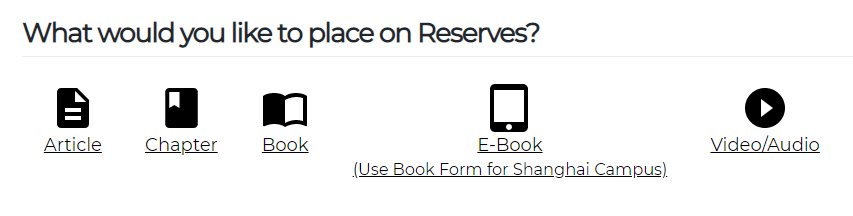
\includegraphics[width=\textwidth]{types}
    \caption{Types of Reserve Items}
    \label{fig: re-type}
\end{figure}
\vspace*{1ex}

\section{Book}
\label{sec:book}
See a full book form on the next page~(\autoref{fig: book form}). To add a book:
% \tcbdocmarginnote{\href{https://youtu.be/wUEl8KrMz14}{video tutorial}}
\begin{itemize}
    \item {\bfseries\uline{Use Book form for both physical book and e-book}}
    \item Make sure the pickup location is Shanghai Library
    \item Add Notes (e.g.\ , things you'd like staff to know), Tags as needed 
    \item Enter N/A if not sure.
    \item Specify if an alternate edition is acceptable and which edition(s), if needed. 
    \item Select how the item will be supplied, two options:
    \begin{description}
        \item[I will bring a personal copy to the library] The material will be provided by you.
        \item[Please have library staff provide the material] The library will process owned material or purchase the material if not owned.
    \end{description}
    \item When finished, click \aresbut{Submit Item}
\end{itemize}

\vspace*{3ex}
\begin{table}[h]
    \centering
    \begin{notebox}
    The fields indicated on the form with an \textcolor{red}{*} are required fields. Please fill out as much information as possible. 
    \tcblower
    As mentioned in \autoref{ch:intro}, {\imp texts are NOT} expected to be submitted through \ares system. Yet if you happen to do so, you may confirm this using the Notes field.
    \end{notebox}
    \label{note: texts not expected}
\end{table}

\vspace*{5ex}
\begin{figure}[h]
    \centering
    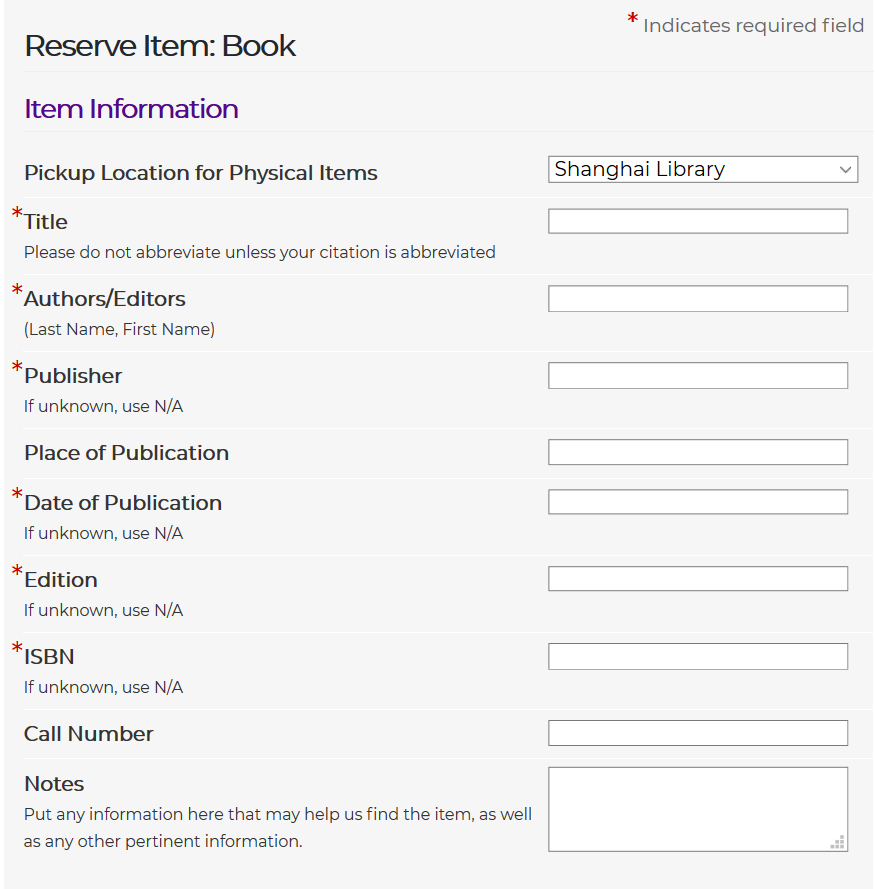
\includegraphics[width=\linewidth]{book1}
    \caption{The Book Form 1}
    \label{fig:bookformone}
\end{figure}


\clearpage
\begin{figure}[h]
    \centering
    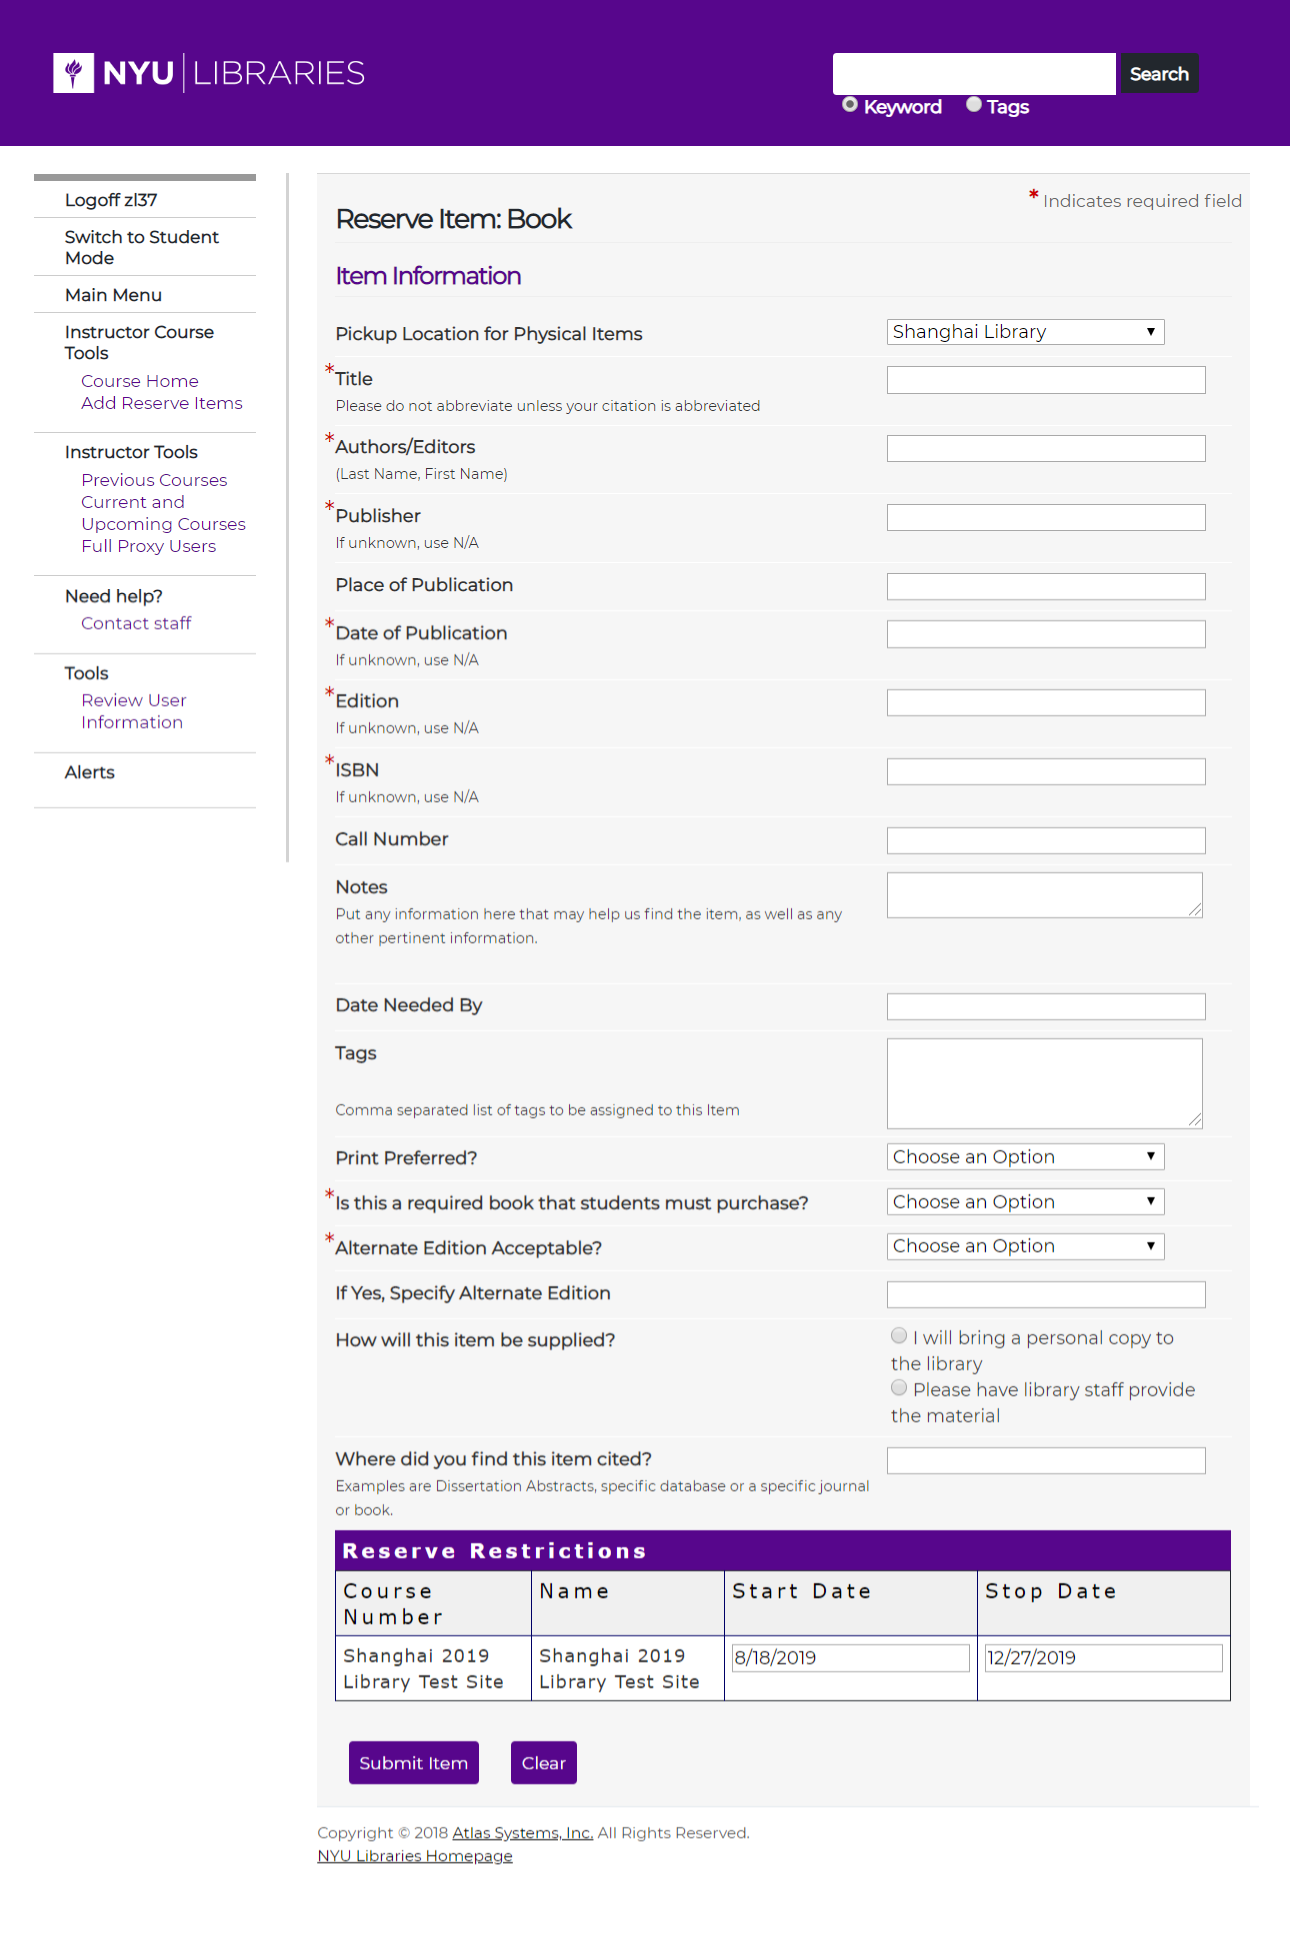
\includegraphics[width=\linewidth, height=22cm]{book}
    \caption{Full Book Form}
    \label{fig: book form}
\end{figure}
\clearpage


\section{Chapter/Article}
\label{sec:bchapterandart}
The forms for these two are very similar. To add a chapter or article:
% \tcbdocmarginnote{\href{https://youtu.be/wUEl8KrMz14}{video tutorial}}
\begin{itemize}
    \item Choose Article if the request is a journal/newspaper article
    \item Choose Chapter if the request is a book chapter
    \item Follow the above steps to fill out the information for book chapter/article item
    \item Add Notes, Tags as needed
    \item Select how the item will be supplied:
        \begin{description}
            \item[I will upload a file] Please be advised the material must be {\imp lawfully obtained and adhere to applicable copyright laws}. \uline{Materials borrowed from Interlibrary Loan SHOULD NOT be placed on E-Reserve without copyright clearance} 
            \item[I will bring a personal copy] The material will be provided by you 
            \item[Please have library staff provide the material] The library will process owned material
            \item[The item should link to a website] The item should link to a website: you will provide a URL
        \end{description}
\end{itemize}

\vspace*{5ex}
\begin{figure}[h]
    \centering
    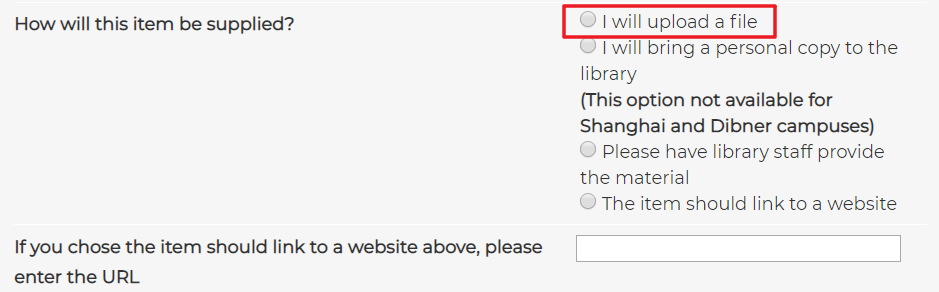
\includegraphics[width=\linewidth]{artpdf}
    \caption{Upload File Option}
    \label{fig:upload artpdf}
\end{figure}

\vspace*{8ex}
\begin{table}[h]
    \centering
    \begin{notebox}
    If you upload an article PDF file, the library staff may replace it with the link to the article, which is more preferable and efficient in \ares system.
    \tcblower
    In terms of uploading a chapter scan (in PDF), please be advised that our guideline is to scan {\imp no more than 2 chapters or 15\% of the whole book, whichever comes first}. For chapter scan, a {\imp Copyright Notice} (see~\autoref{ch:copyright}) is needed at the very beginning of the scan.
    \end{notebox}
    \label{note: guideline}
\end{table}


\clearpage
\begin{figure}[h]
    \centering
    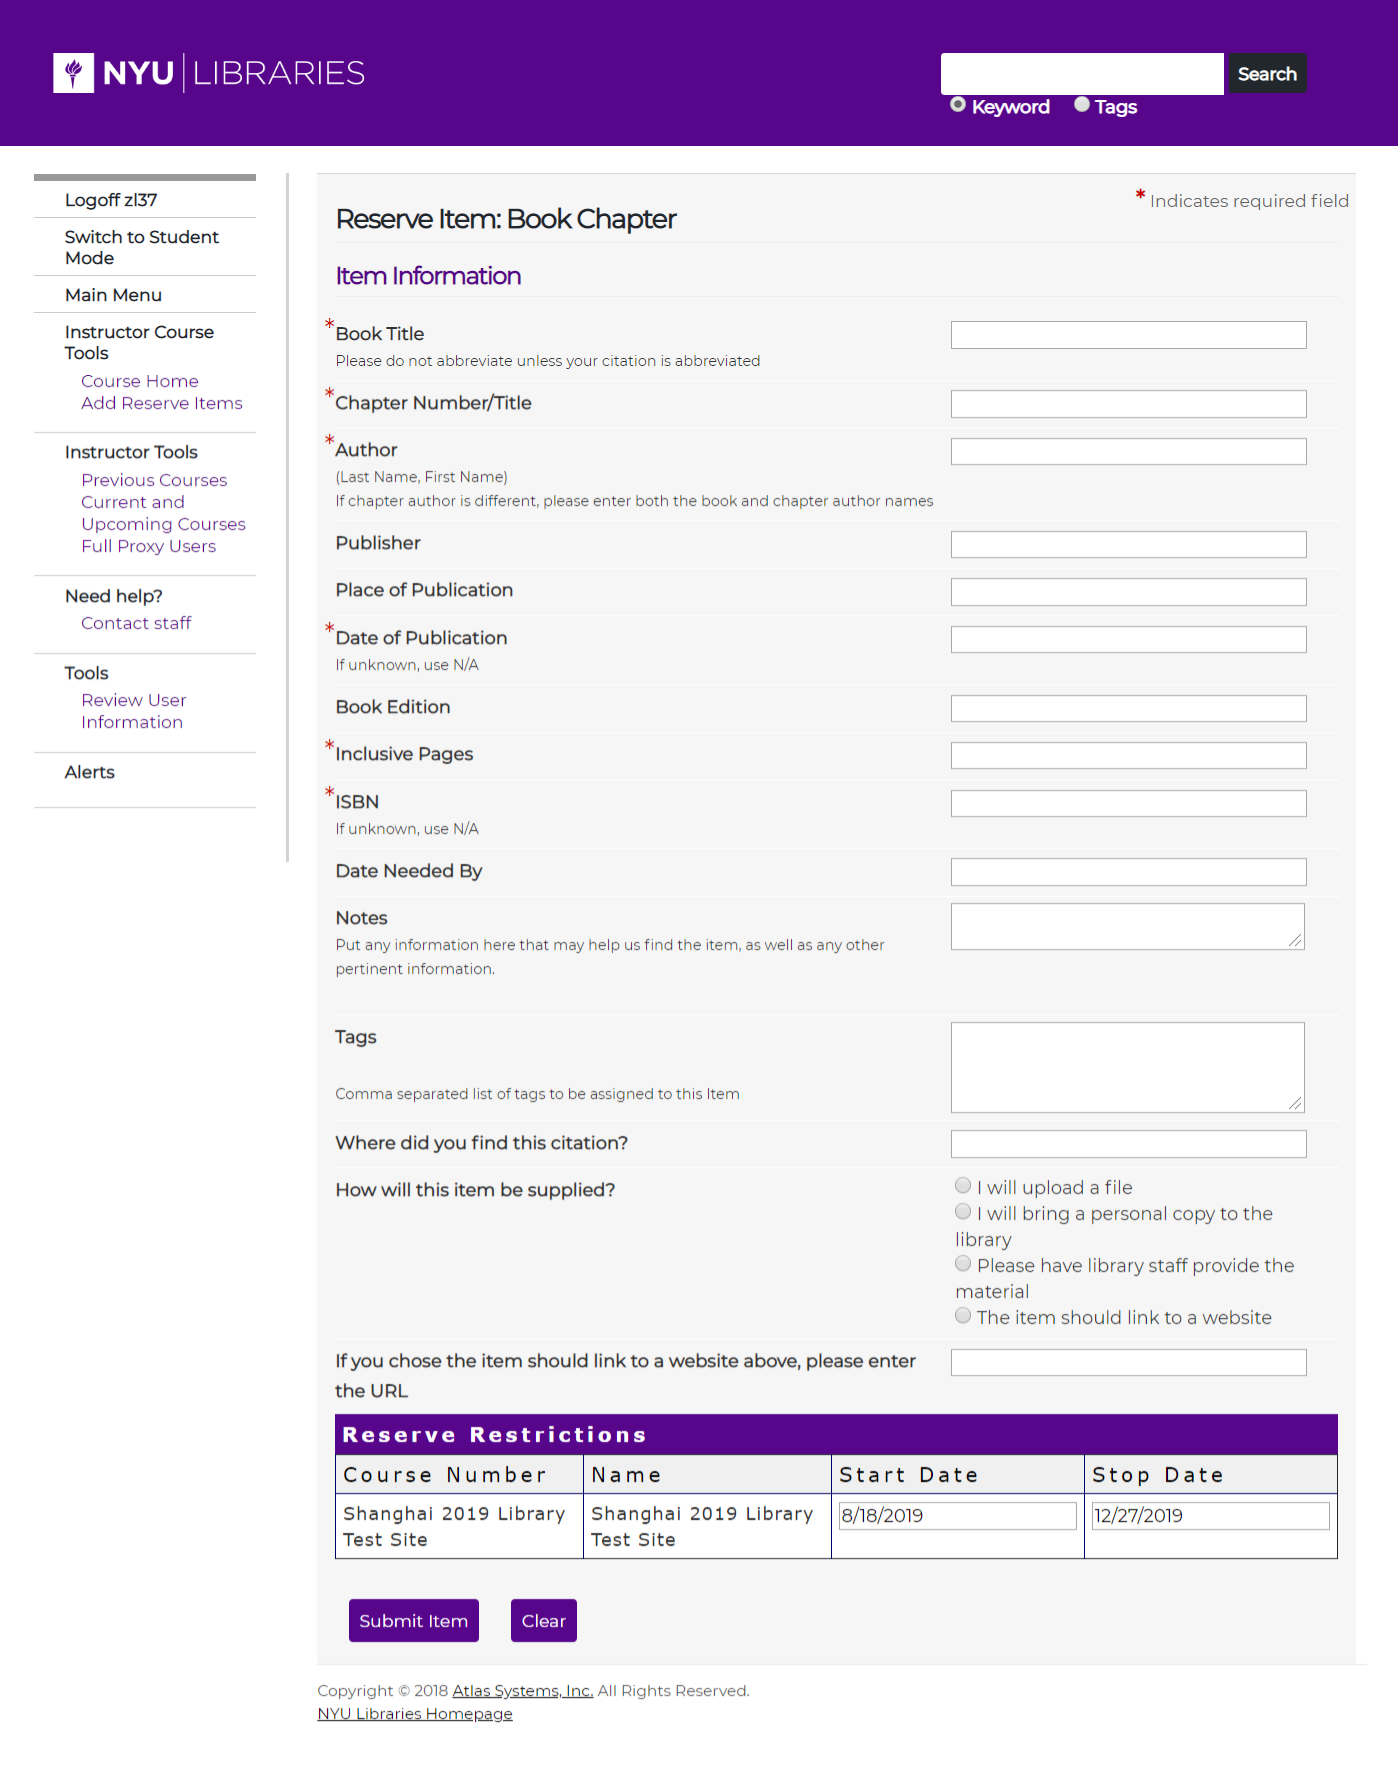
\includegraphics[width=\linewidth, height=22cm]{bookchapter}
    \caption{Full Book Chapter Form}
    \label{fig: chapter form}
\end{figure}
\clearpage

\clearpage
\begin{figure}[h]
    \centering
    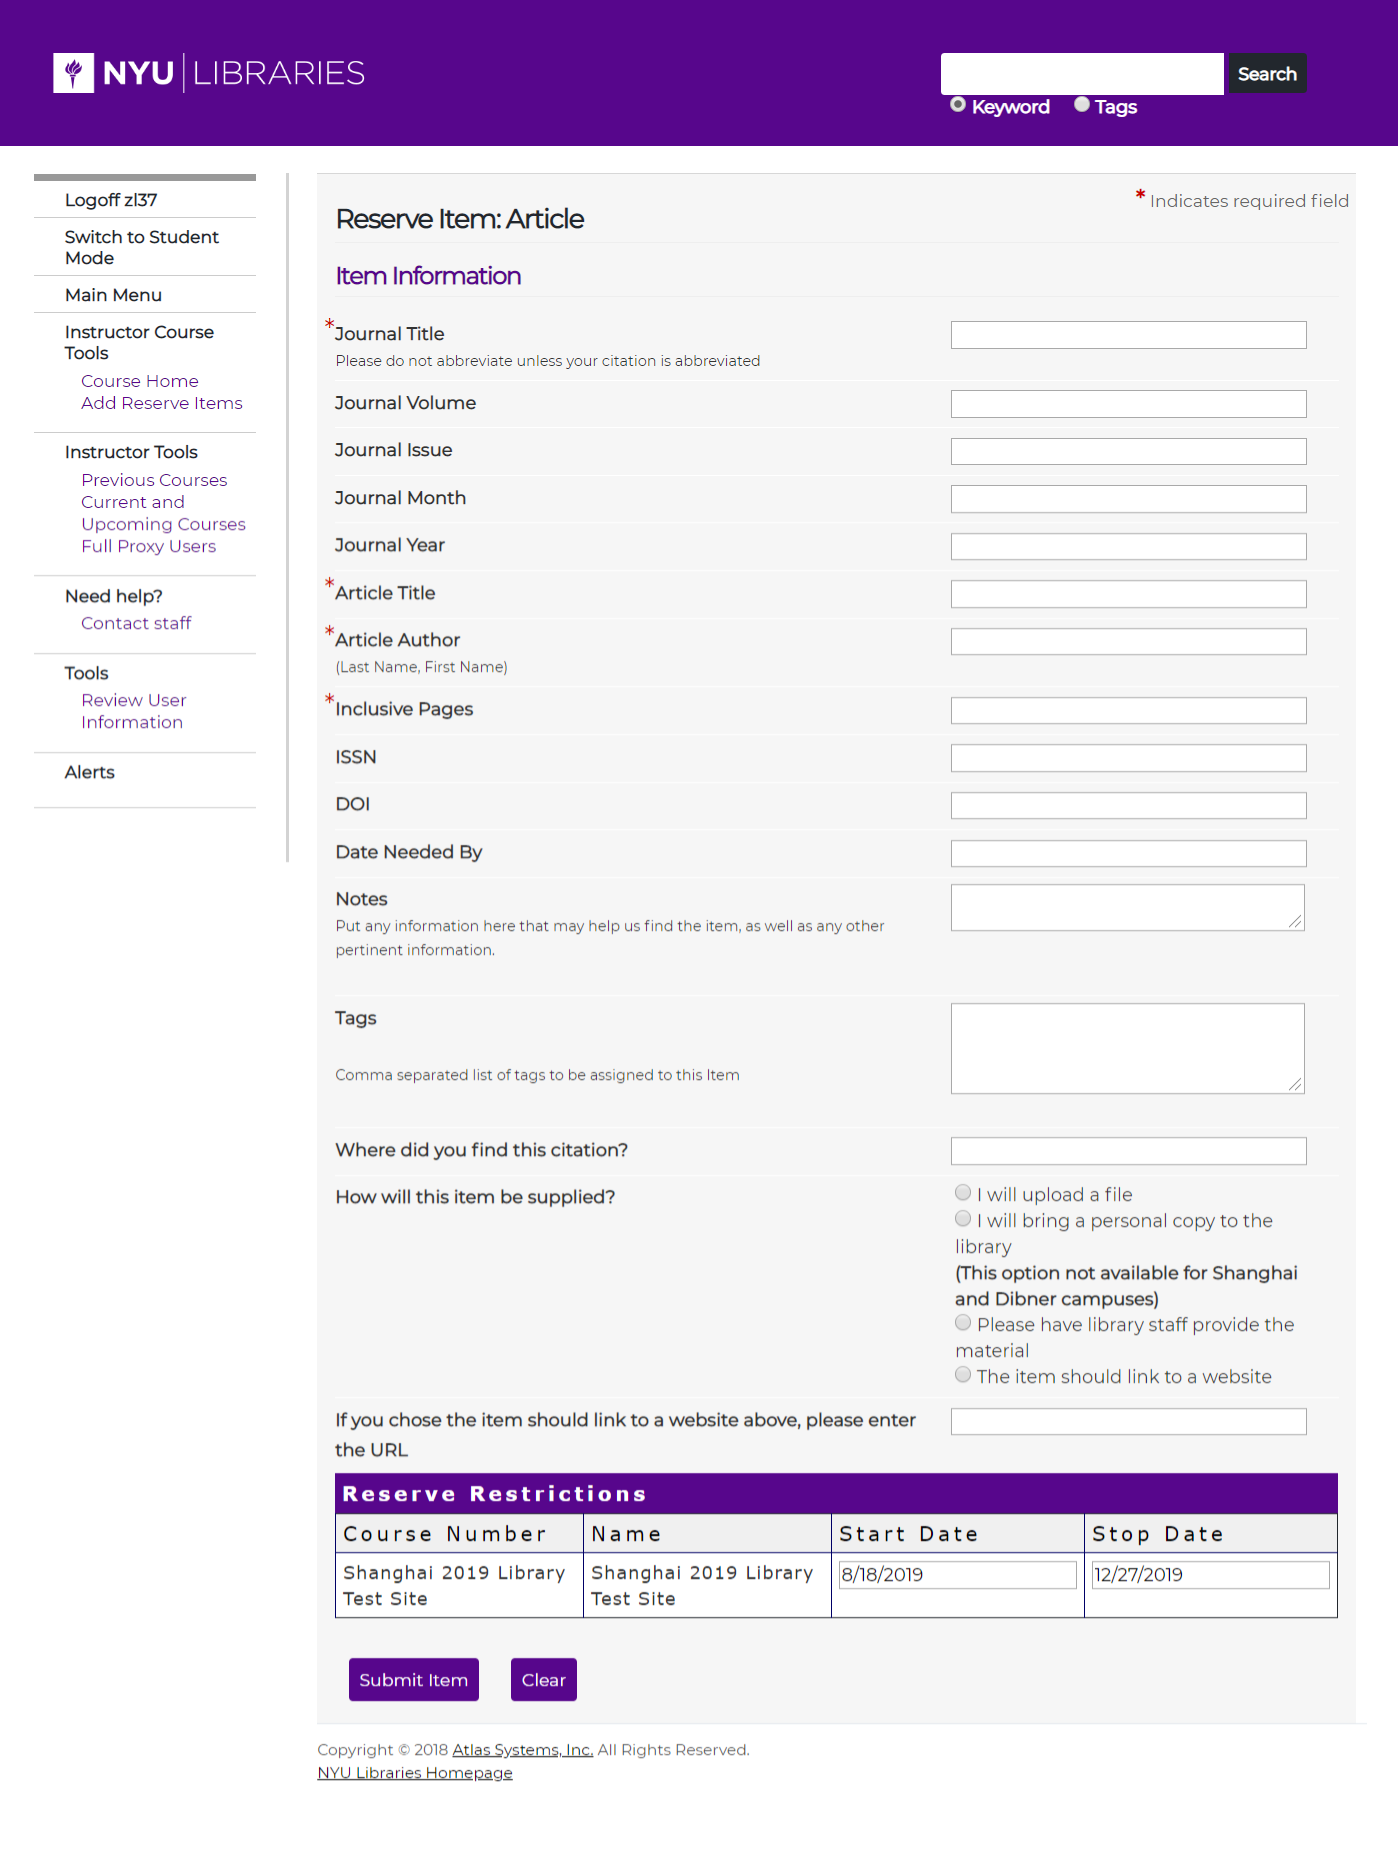
\includegraphics[width=\linewidth, height=22cm]{article}
    \caption{Full Article Form}
    \label{fig: article form}
\end{figure}
\clearpage



\section{Video}
\label{sec:video}
To add a video is quite straightforward, though it's better to explain a bit about the following two fields:
% \tcbdocmarginnote{\href{https://youtu.be/wUEl8KrMz14}{video tutorial}}
\begin{description}
    \item[\textcolor{red}{*}Select an item type] You can select from Video, Audio or Other Media. ``Audio'' usually refers to VCD. If you choose ``Other Media'', please do let the library staff know what you are referring to by putting some explanation in the \textbf{Notes} field.
    \item[\textcolor{red}{*}Call Number] You can first do a quick search via \href{https://shanghai.nyu.edu/academics/library}{BobCat}. If the video you need happens to be in the library's Media Collection, you will find one (e.g.\ DVDSH 1230). Of course, you can just put ``NA'' there. 
\end{description}

\vspace*{5ex}
\begin{figure}[h]
    \centering
    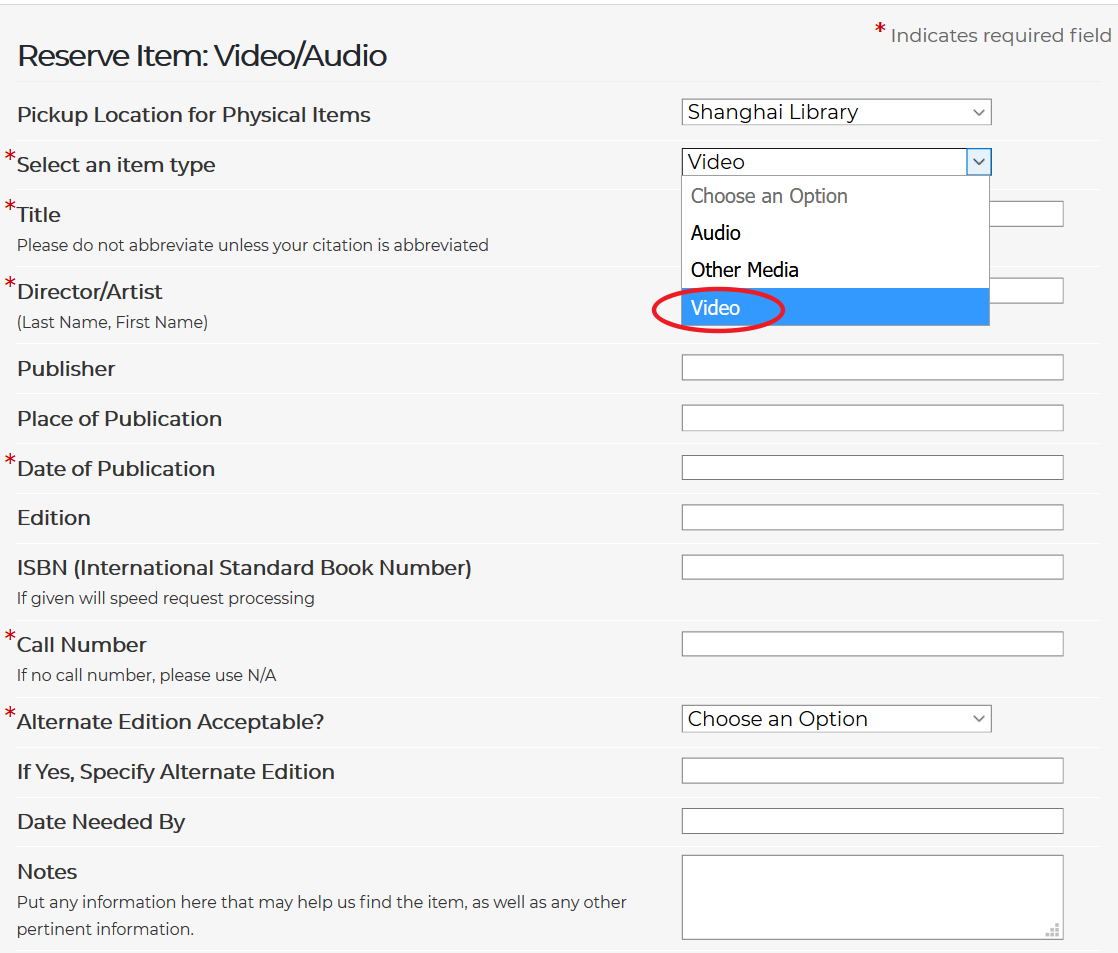
\includegraphics[width=\linewidth]{video1}
    \caption{Video Form}
    \label{fig:videoform}
\end{figure}


\clearpage
\begin{figure}[h]
    \centering
    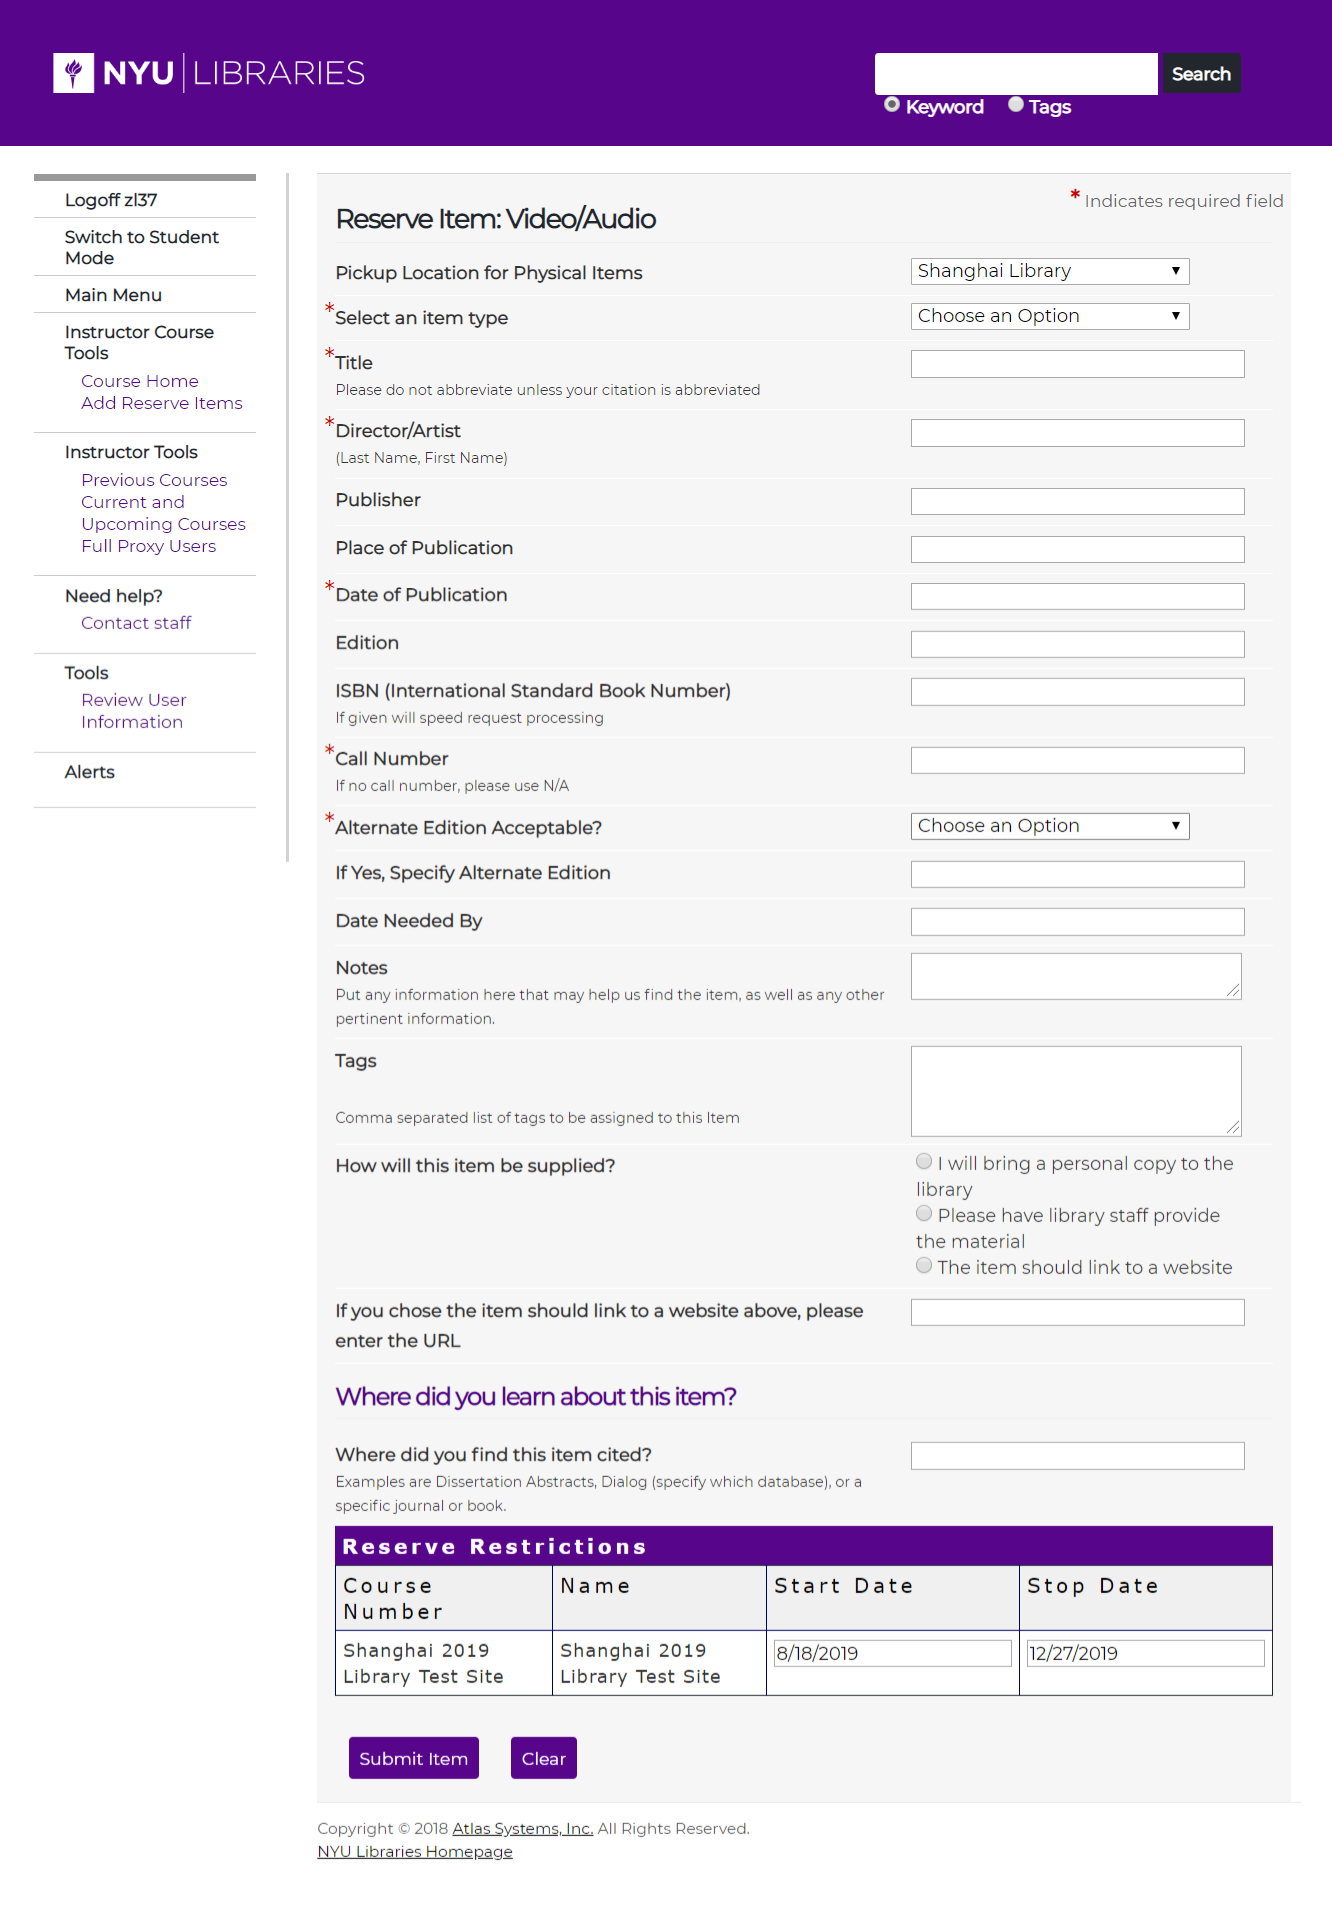
\includegraphics[width=\textwidth]{video}
    \caption{Full Video Form}
    \label{fig: video form}
\end{figure}
\clearpage
